\chapter{Úvod}
Vývoj centrálního zásobování teplem prošel od dob svého vzniku několika fázemi.
Z hlediska dnešní doby je nejvýznamější býměna starých parovodů za
prefabrikované horkovody, čímž dochází ke snížení přestupu tepla z rozvodů do
jejich okolí a snížemí nákladů při stavbě nových částí sitě. Z hlediska
několika budoucích dekád je žádoucí transformace na obnovitelné, plně
udržitelné a efektivní zásobování teplem. To přináší nové technologické výzvy
související zejeména s integrací obnovitelných zdrpjů, využitím odpadního tepla
a celkově snižováním emisí oxidu uhličitého. Je totiž obecně přijímaným faktem,
že pro smysluplnou implementaci obnovitelných zdrojů tepla a odpadní, jež lze
obecně lze obecně považovat za nízkoteplotní zdroje, je nutné dále snižovat
teplotu v teplárenských rozvodech. Snižovaní této teploty má za následek další
redukci ztrát při distribuci tepla, ale komplikuje efektivní předávání tepla na
straně spotřebitelů a zvyšuje provozní náklady čerpadel. Proto je nutné do sítě
implementovat další prvky, jež umožní efektivní zvýšení teploty blízko
samotných spotřebitelů. Jako další problém lze zmínit značnou nestálost
obnovitelných zdrojů tepla. Se zvyšující se komlexností sítí bude nutné zlepšit
možnosti optimalizace jejich provozu. Toho lze dosáhnout například prediktivním
řízením využívající matematické modely a vhodnou koncepcí akumulace tepla
společně s předpovědí počasí a predikcí množství potřebného tepla. Systémy, jež
se budou schopny vypořádat s těmito a dalšími výzvami lze obecně nazvat čtvrtou
generací teplárenských sítí \cite{Lund2014}.

Množství hmoty, které ovlivňuje fyzikální dynamiku rozsáhlých energetických
systémů již samo o sobě naznačuje komplexnost potencionálního matematického
modelu (digitálního dvojčete či prototypu). Užitečnost takových modelů roste
společně s jejich výpočtovou rychlostí a také s rychlostí s jakou je možné tyto
modely sestavovat. Deklarativní programování může výrazně zjednodušit proces
kompletace z jednotlivých komponent. V numerickém řešení pak modely obvykle
využívají matice, jež se v nich objevují zpravidla kvůli tzv. linearizaci
diferenciálních rovnic (tedy rovnic řídících fyzikální chování). Výpočtová
rychlost je pak úměrná velikosti a hustotě těchto matic. V dnešní době se
můžeme často setkat se snahou o zmenšováním matic pomocí redukce směrem k tzv.
jedno‑dimenzionálním modelům. Dalším výrazný vliv na výpočetní rychlost mají
programovací jazyk použitý pro implementaci (strojový kód zpravidla poběží
rychleji než kód interpretovaný) a také míra a provedení paralelizace
algoritmů.

Počítačové učení je moderní vědecká disciplína, která umožňuje vytvářet modely
pomocí dat a to na základě optimalizace parametrizovaných programů. V této
oblasti existuje celá řada numerických struktur umožňující až univerzální
aproximaci (např. neuronové sítě).

Cílem této disertační práce je vytvoření nástrojů (softwarových balíčků) pro
modelování komponent tepelného zásobování s ohledem na optimalizaci numerické
efektivnosti simulací s využitím deklarativního programování a počítačového
učení. Model tepelného zásobování zde poslouží jako studijní příklad jejich
aplikace.

\chapter{Abstrakt}
\label{abstrakt}
Text abstraktu.

\chapter{Současné shrnutí stavu poznání}
\label{struktura}
V této kapitole je provedena rešerše problematiky modelování CZT a popis
vybraných matematických rovnic aplikovatelných pro daný kontext. Dále jsou
popsány použitelné výpočetní přístupy spolu s aspekty, ovlivňující numerickou
efektivnost.

\section{Stručná historie rozvoje teplárenství}
\label{sec:history}
Teplárenské potrubí slouží k dopravě tepla od jeho výrobce k jeho spotřebiteli
pomocí teplonosného média. V minulosti se jako první teplonosné médium
používala pára o teplotě i přes 240 °C. Tyto rozvody generovaly značné tepelné
ztráty a kvůli vysokému tlaku (naakumulované tlakové energii) i váž:né
explozivní nehody. Kvůli kondenzaci páry ve vratném potrubí docházelo k jeho
korozi. Pára se jako hlavní teplonosné médium stále využívá například v Paříži
či Manhattanu. Nástupce tohoto provedení využíval tlakovou horkou vodu většinou
přes 100 °C. Kvůli nestlačitelnosti vody se výrazně omezily explozivní nehody.
Motivací bylo snížení tepelných ztrát a možnost lepší implementace kombinované
výroby tepla a elektrické energie v městských oblastech. Poté přišel trend
snižování teploty v rozvodech pod 100 °C. Stále byla využívána tlaková horká
voda. Začalo se značně využívat prefabrikované a před-izolované potrubí
snižující množství lidské práce při výstavbě a obnově rozvodů. Začala se
využívat lokální paliva, odpady a na několika místech i sluneční či geotermální
energie. V následujících dvou až třech dekádách bude trend snižování teploty v
rozvodech pokračovat ruku v ruce se snižující se náročností budov na prostorové
vytápění. Bude existovat snaha o výraznější implementaci obnovitelných a
odpadních zdrojů energie a k využívání synergií. Pro snížení následků fluktuací
zdrojů, budou využívány akumulační systémy společně s prediktivním řízením
využívající předpovědi meteorologických podmínek a matematické modely
jednotlivých součástí systému se zaměřením na jejich dynamiku \cite{Lund2014}.

\section{Tepelná dynamika teplárenských rozvodů/potrubí}
\label{sec:HeatDynamics}
Moderní teplárenské systémy s teplonosným médiem v kapalném skupenství. Fluidní
dynamika je prostorovým fenoménem, ale lze zavádět zjednodušující předpoklady
odpovídající kontextu aplikace. Při uvažování zjednodušené fyziky proudění
tekutiny v potrubí (tj. na nestlačitelné a jedno-dimenzionální proudění) lze
problém zjednodušit na součinnost třech fyzikálních jevů:

\begin{itemize}
\item Advekce veličin jež jsou unášeny proudem podél potrubí
\item Difůze veličin v tekutině podél potrubí
\item Příspěvky do veličin vnitřními a/či externími zdroji
\end{itemize}

\begin{figure}[h] \capstart
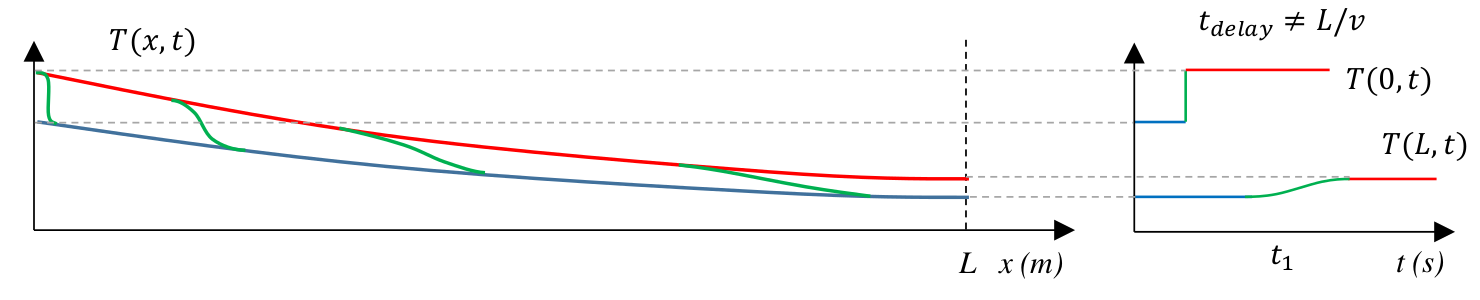
\includegraphics[width=\textwidth]{figures/heat_front}
\caption{Proces šíření teplotní vlny v potrubí \cite{Abraham2009}}
\end{figure}

Parciální diferenciální rovnice (PDR) pro celkovou dynamiku je pak v tomto
kontextu následující:
\begin{equation}
  \label{eq:AdvDiff}
  \frac{dy}{dt} = -u \frac{dy}{dx} + D\frac{d^{2}y}{dx^2} + {S_y}
\end{equation}
kde \(y\) je unášená veličina, \(t\) je čas, \(x\) je podélná poloha, \(u\) je
rychlost tekutiny, \(D\) je celkový koeficient difúze a \(S_y\) je celkový
zdroj unášené veličiny. Z hlediska tepelného chování může být touto veličinou 
měrná entalpie, ale lze pracovat i s teplotou.

Advekce je jev, při kterém se transportují veličiny (jsou unášeny) ve směru
objemového pohybu. Tento jev ovlivňuje tepelnou dynamiku nejvíce, neboť z velké
části určuje čas transportu (zpoždění) teplotní fronty.

Intenzita axiální difúze (velikost koeficientu D) je složena jednak z difúze
kodkukcí tepla v tekutině a dále z efektu tzv. turbulentního míchání v axiálním
směru. Difúze způsobená kondukcí je u teplárenských rozvodů zanedbatelná
\todo{cite}. Za to turbulentní difúze roste dle přibližně lineárně s
Reynoldsovým číslem \todo{cite}. Axiální difúze způsobuje rozpínání
(vyhlazování) teplotní fronty, což znamená, že náhlé změny na vstupu do potrubí
se projevují pozvolnými změnami na jeho konci. V případě uvažování horizontálně
uloženého potrubí lze tímto způsobem zahrnout i vliv gravitace. Nemá tak vliv
na zpoždění teplotní fronty, ale výrazně ovlivňuje její tvar.

Zdrojový termín \(S_y\) zahrnuje především výměnu tepla mezi tekutinou a
vnitřním povrchem přilehlé stěny ve kterém tekutina proudí (což v důsledku
určuje vliv akumulace tepla na vývoj teplotní fronty). Velikost hustoty
tepelného toku je závislá na rozdílu teploty vody a povrchu, vlastnostech
tekutiny, velikosti a drsnosti povrchu a na rychlosti proudění. Výměna tepla
ovlivňuje jak zpoždění teplotní fronty tak její tvar. Intenzitu výměny tepla
lze vyjádřit obyčejnou rovnicí konvekce tepla \ref{eq:ConvHeatTransfer}.

\begin{equation}
  \label{eq:ConvHeatTransfer}
  Q = \alpha S \Delta T
\end{equation}
kde \(Q\) je tepelný tok ze stěny do tekutiny,\(\alpha\) je součinitel přestupu
tepla, \(S\) je velikost plochy kde je styčného povrchu a \(\Delta T\) je
rozdíl teplot povrchu a tekutiny. Koeficient přenosu tepla  je možné určovat z
tzv. Nusseltova čísla, které vyjadřuje poměr mezi konvektivním a koduktivním
přestupem tepla. Známe-li tedy množství tepla, jež by procházelo mezní vrstvou
v případě čisté kondukce tepla je možné určit množství tepla v případě
konvektivního přestupu tepla:

\begin{equation} 
  \label{eq:NusseltDef}
  Nu = \frac{\alpha L}{\lambda} 
\end{equation}
kde je \(Nu\) Nusseltovo číslo, \(L\) je charakteristický rozměr (pro kruhové
potrubí je jím vnitřní průměr) a \(\lambda\) je tepelná vodivost tekutiny.

\begin{figure}[h] \centering \capstart
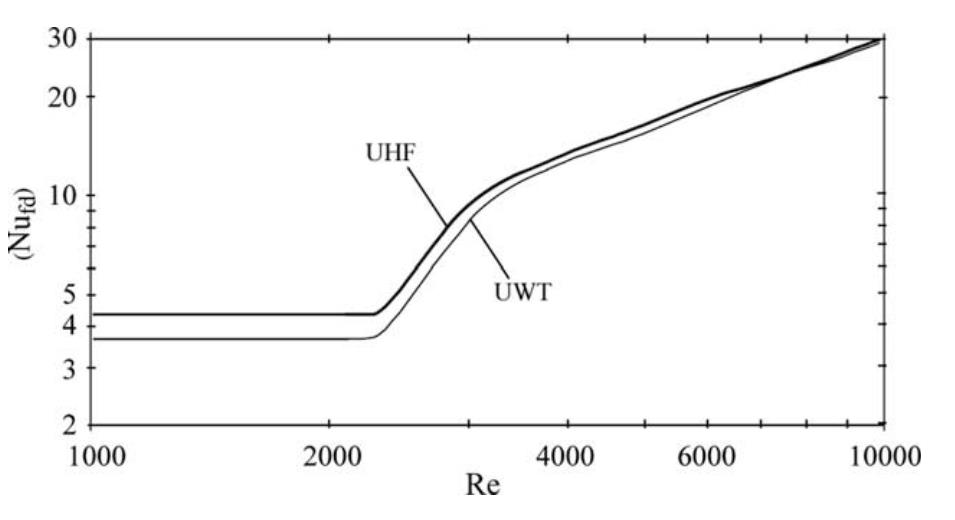
\includegraphics[scale=0.3]{figures/nusselt}
\caption{Závislost Nusseltova čísla na Reynoldsově čísle \cite{Abraham2009}}
\label{fig:NuReynolds}
\end{figure}

Hodnotu Nusseltova čísla je možné určit na základě vztahů jak pro rovnoměrné
rozložení teploty na stěně (označováno jako UWT), tak pro rovnoměrné rozložení
tepelného toku (označované jako UHF). Dle \cite{Abraham2009} je pro všecny
režimi proudění vhodné používat následující model Nusseltova čísla:
\begin{equation}
\label{eq:NuModel}
  Nu =
  \begin{dcases}
    c_0 & Re\leq 2300 \\
    \sum_{i=1}^{5} c_i\left(\frac{Re}{10^3}\right)^{5-i} & 2300 < Re\le 3100 \\
    \frac{\frac{f}{8}(Re-1000)Pr}
    {1+12.7{\frac{f}{8}}^{(1/2)}(Pr^{(2/3)}-1)} & 3100 < Re
  \end{dcases}
\end{equation}
kde \(Pr\) je Prandtlovo číslo (vlastnost tekutiny) a \(f\) je Darcy-Weisbachův
koeficient tření který je popsán v podkapitole \todo{ref section} (skrze něj
se projevuje vliv drsnosti). Jednotlivé hodnoty parametrů tohoto modelu jsou:
\begin{table}[H]
  \label{tab:NuModel}
  \caption{Parametry modelu Nusseltova čísla}
  \vskip6pt
  \centering
  \begin{tabular}{ccc}
    \toprule
    Parameter & UWT & UHF \\ [0.5ex]
    \hline
    \(c_0\) & 3,66 & 4,36 \\
    \(c_1\) & 3,52 & 2,2407 \\
    \(c_2\) & 45,148 & 29,499 \\
    \(c_3\) & 212,13 & 142,32 \\
    \(c_4\) & 427,45 & 292,51 \\
    \(c_5\) & 316,08 & 219,88 \\
    \bottomrule \\[0.1mm]
  \end{tabular}
\end{table}
V případě, že je teplota vnitřního povrchu potrubí známa je možné na základě
rovnic \ref{eq:ConvHeatTransfer} až \ref{eq:NuModel} určit intenzitu výměny
tepla v konkrétním okamžiku. Tato teplota je však ovlivněna tepelnou hmotou jež
obklopuje fluidní region (např. ocelová trubka, izolace, zemina apod.) a tudíž
je nutno korektně matematicky zachytit \todo{ref-solid model}.

\section{Fluidní region - tlakové ztráty/akcelerace tekutiny}
\label{sec:PressureLoss}
Tlakové vlny se v potrubí šíří výrazně rychleji (rychlostí zvuku) než vlny
teplotní (přibližně rychlost proudění tekutiny), což znamená že lokální
události probíhají v daleko kratším časovém měřítku. Z tohoto důvodu je potřeba
v immulacích s tlakovými pulsacemi využívat krátký časový krok. Predikce
tlakových vln je užitečná pouze z hlediska ochrany proti poškození způsobených
tlakovými rázy a na vývoj distribuce tepla nemá výraznější vliv.
Při zandebání rychlých tlakových pulsací lze akceleraci tekutiny podél potrubí
modelovat pomocí následující PDR:

\begin{equation}
  \label{eq:momentum}
  \frac{du}{dt} = -\frac{dp}{dx} - \frac{1}{2}\frac{f}{D}u|u|
\end{equation}
kde \(\rho\) je hustota tekutiny (závislá na teplotě), \(p\) je tlak a \(D\) je
vnitřní průměr potrubí. Hodnotu třecího koeficinetu \(f\) lze určit z
explicitní Churchilovy rovnice \ref{eq:Churchill} \todo{cite}, která je
relativně přesná pro všechny režimy proudění.

\begin{equation}
  \label{eq:Churchill}
  \begin{gathered}
    f=8\left(\left(\frac{8}{Re}\right)^{12}+(A+B)^{-1.5}\right)^\frac{1}{12} \\
    A=\left(2.457\ln\left(\left(\frac{7}{Re}\right)^{0.9}
      +0.27\frac{\epsilon}{D}\right)^{-1}\right)^{16} \\
    B=\left(\frac{37530}{Re}\right)^{16}
  \end{gathered}
\end{equation}

\section{Okolní hmota – kovová stěna, izolace, zemina}
\label{sec:SurroundingMass}
Pro popis vedení tepla v okolí fluidního regionu potrubí je vhodné využít
obecnou PDR vedení tepla \ref{eq:HeatEq} v obecném \(\mathcal{R}^n\) prostoru.
\begin{equation}
  \label{eq:HeatEq}
  \frac{dT}{dt}\rho{c_p}=\nabla(\lambda\nabla{T})+S
\end{equation}
kde \(\rho\) je hustota, \(c_p\) je měrná tepelná kapacita, \(\lambda\) je
tepelná vodivost, \(T\) je teplota a \(S\) je zdroj tepla. Tato rovnice platí
pro všechny souřadnicové systémy, jelikož pro každý souřadnicový systém
existuje konkrétní rozvin operátoru \(\nabla\).

\section{Vlastnosti média a materiálu}
Vlastnosti tekutiny a materiálů jež vystupují v rovnicích \ref{eq:AdvDiff} až
\ref{eq:HeatEq} jsou ve skutečnosti závislé na teplotě a na tlaku (nebo
obecněji na stavových veličinách). Existují implementace programů mezinárodní
asociace pro vlastnosti vody a páry (IAPWS) \todo{cite IAPWS}, které popisují
vlastnosti vody a páry velmi přesně. Při uvažování nestlačitelnosti vody jsou
vlastnosti jako hustota, či viskozita stále výrazně proměnlivé s teplotou. Pro
tuhé skupenství je zpravidla dostačující popis polynomiální funkcí nebo i
konstantou. Při popisu zeminy se může výrazně projevit vliv její vlhkosti, což
znamená že její vlastnosti jsou proměnlivé v čase.

\begin{figure}[h] \centering \capstart
  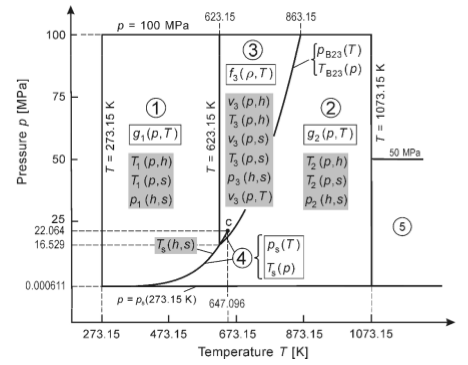
\includegraphics[scale=0.7]{figures/IF97}
  \caption{Regiony implementace vlastností vody a páry IF97 \todo{cite IAPWS}}
  \label{fig:IF97}
\end{figure}

\section{Numerické řešení a rychlost simulací}
\todo{OpenSource proč – dostupnost vědecké komunitě, cutting edge atd}

V rovnicích \ref{eq:AdvDiff}, \ref{eq:momentum} a \ref{eq:HeatEq} vystupují
diferenciální operátory a zejména tyto jsou fundamentálně příčinnou numerické
náročnosti simulací. I přesto, že je fyzika popsaná v sekcích
\ref{sec:HeatDynamics}, \ref{sec:PressureLoss} a \ref{sec:SurroundingMass} je
výrazně zjednodušena, je stále nutné diskretizovat v prostoru a čase
(linearizovat problém). Lze využít metody jež jsou určeny a optimalizovány
přímo pro daný kontext. Například pro rovnici \ref{eq:AdvDiff} lze využít
integrační metody vyvinuté v NASA, které využívají aproximace derivací vyšších
řádů nežli je definováno v samotné PDR. Takových řešení lze nalézt např. v 
\todo{cite leonard}, kde jedním znejefektivnější schémat je ULTIMATE QUICKEST.

Velmi častý postup při řešení PDR je její převedení na systém ordinárních
diferenciálních rovnic (ODR), jež je dále integrován (simulován) v čase pomocí
separátních algoritmů. PDR jsou v prostoru nejčastěji linearizovány pomocí
metody konečných diferencí (MKD), metody konečných objemů (MKO) či metody
konečných prvků (MKP). Pro sestavení matic a následnou integraci v čase
existuje celá řada komerčních nástrojů s přednastavenými řešiči pro jednotlivé
systémy PDR. Z Open-Source projektů zabývajícími se automatizovaným řešení PDR
je vhodné  zmínit FeniCS \todo{cite FeniCS}, kterým je možné řešit PDR pomocí
MKP (umožňuje i tzv. nespojitou Galerkinovu metodu jež kombinuje vlastnosti MKP
a MKO a je vhodná i pro fluidní dynamiku). Tato knihovna umožňuje velmi 
detailně kontrolovat jakým způsobem jsou sestavovány matice, jaké konečné 
elementy jsou využívány, jakým způsobem bude během výpočtů manipulováno s 
objekty lineární algebry a mnoho dalšího.

Výsledkem procesu linearizace je systém lineárních rovnic z pravidla
reprezentovaný v maticové formě (tj. lineární algebra). Velikost a hustota 
(podíl nenulových hodnot) těchto matic pak přímo ovlivňují rychlost simulace, 
neboť přímo korespondují s počtem CPU cyklů, které musí procesor (či procesory)
využít na aritmetické operace během jednoho časového kroku. V případě, že je
výsledný systém nelineární (např. jsou-li tepelné vlastnosti závislé na
teplotě) je tento vliv ještě umocněn. Pro integraci v čase existují explicitní
či implicitní algoritmy s konstantním nebo adaptivním časovým krokem. Jedny z
nejefektivnějších algoritmů jsou součástí knihovny SUNDIALS
\todo{cite sundials}, která je implementována v jazyce C.
\label{kapitoly}


\textbf{Příklad}:
\begin{verbatim}
   @Article{Cech:2020:Citace,
	   author               = "Čech, Jan",
	   key                  = "Cech",
	   ... 
\end{verbatim}


